\chapter{Introduction}  \label{ch:intro}

%Introduce the general area of interest that the contents of the review deal with, setting out any advancements and challenges of interest. Then introduce more fully the specific topic addressed in the review and you can then to go on to state any main aim or objectives to be met. Say very briefly what is to come in the layout of the review. Note: the Introduction should include general references to back up the points made.
% Establishing the field
%Definition:
%What are the Olympic classes sailing?
%How are the competitions setting  up?
%What does position and direction means?
%What time steps are you referring for the wind forecast, which sizes?

%Add significance of the main question be sure this was explained properly 
In recent years the integration of new technologies on training programs of professional athletes have been increased. Not only to enhance their motor skills, and to prevent injuries but also to obtain better results with minimal time and in a more efficient process. For example, the use of information that specifies the conditions or parameters that deliver the best results to win, have gained more popularity within the sports community. The involvement of science like kinesiology \cite{sjogaard2015science}, movement science; and engineering is not only concentrated in the athletes but in the elements and factors that cannot be controlled by them, but by those that impact their results. One of these sports is sailing where athletes have to guide the sailboat under different weather conditions and where time is crucial to winning the race.\par
During sailing races such as coastal, inland waterways and lakes, athletes are not allowed to get any information from coaches during the race; for this reason, their preparation and training are not only physical. During training, they acquire skills to anticipate the weather changes and at the same time maneuvers to improve the performance of the sailboat. \par
%For example, a well know competition and classes are the Olympic sailing competitions which take place on coastal and improvements on the boat are not allow. \\
In this section, the research problem, its relevance, and the objectives are going to be presented. For this, a brief definition of Olympic sailing classes and courses are going to be explained followed by an explanation of the information considered by the coaches and athletes to plan the strategy before the competition takes place which most of the time refers to the weather forecast. These data provide a framework to set-up the assumptions and limitations considered in this research. \par 
\section {Olympic Sailing} \label{sec:olympic classes}
The Olympic Sailing Classes are characterized by the rule of a one-design boat. Each class is defined by the sailboat to use; type, size of the hull, number of sails, area, and style, the size of the crew and the gender of them.  The intention of this is to leave out the influence of technology on the results and to focus on the abilities of the athlete to perform effectively; for this reason, the scope for many types researches is on the athlete only. Figure \ref{fig:olymp_cla} shows the names and categories of the current classes that the International Federation of sailing defines as Olympic Classes. The list is subject to change and it is reviewed every 4 years when the Olympic Games have been completed.\par 
The dinghy is not only the smallest and simplest sailboat, one sail and one hull, propelled by wind, but the one used in most of the classes. The differences between their classes rely on the dimensions of the boat and sail, despite using the same type of boat, these differences impact on the speed of the boat and maneuverability. The dimensions on the hull and sails are determined by the number of crew members,1 or 2, and their gender. This research is going to use the dinghy as a reference boat; because is the simple boat, one hull one sail, used extensively on the Olympic Classes. Another reason is due to its similarity physically and mathematically with yachts which have been studied since 1979 \cite{marchajaereo1979}, this allows that some approaches and information can be taken or borrow from them, either to compare or validate the results obtained.\par 

\begin{figure}[ht]
\centering
 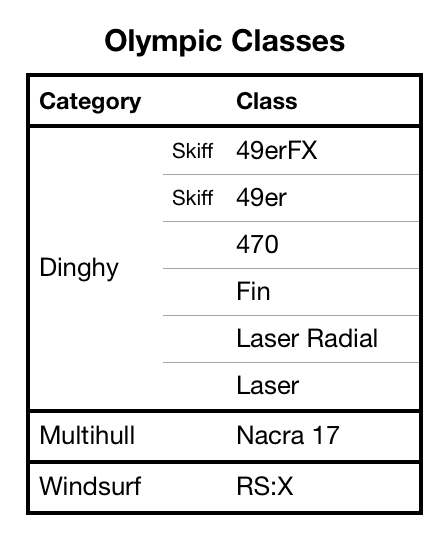
\includegraphics[width=0.32\textwidth]{olym_classes.png}
  \caption{Olympic classes \cite{sailoly}.}
\label{fig:olymp_cla} 
\end{figure}

The competition in each class stands for many races and days where the configurations of the course vary according to the environmental conditions. In each race, points are given according to its arrival position; the faster, the lower the score. The winner is the one with the lowest score. Under this competing format, athletes and coaches confront distinct scenarios for which they take different decisions at the starting line. One of these decisions refers to the initial sailing direction. Its importance is related to the configuration of the course.\par 

\section{Competition Course}\label{tracks}
The most common form of a sailing competition is the fleet racing where all participants race around a course and start at the same time along with a line. Here, not only is the reaction time important but the direction that allows the maximum speed that could be attained is too. Usually, two different types of courses take place in the Olympic classes. Figure \ref{fig:trap_c} shows the singular trapezoid course which is defined by a separate start and finish line and 4 points around (buoys); these 6 elements define the legs of the competition, the first leg is the longest one and it is running against the wind.
The trapezoid course is the most completed format courses, the other formats are a partial representation of it, considering only some legs which are already represented in the trapezoid course.\par 
%The other course is the windward/leeward, figure \ref{fig:wl_c} this is simply a two-leg race orientated in such way that the first leg is sail against the wind (called a beat) and the second leg is sail with the wind (called a run). If boats are sailing neither with nor against the wind, the leg is called reach. 

The courses characteristics and conditions of race are also subject to change every 4 years. For example, the current course is regulated as follows \cite{race_pol}: The length and angles of each leg are defined in such way that the course could be completed in maximum 1 hour and the trapezoidal course can be contained in a grid size of 2km by 2km.  Another consideration is the area of the course,  which most of the time is expressed in nautical miles (nm).Figure \ref{fig:olymp_areas_rio} is an example of how the sailing areas are defined by a circular area, within this circle the trapezoid should be located. \par 
Furthermore, the wind conditions refer to the average wind speed in addition to its shift direction. The current regulation establishes that the race will not start if the average wind speed is less than 4 knots(kn)[2 m/s] or more than 25 knots(12.86 m/s) over the entire course, with maximum wind shift of 10$\deg$. 
If wind conditions are not meet the race could be delayed, and if the race has already started, it is possible a change in the course or an abandonment of the race \cite{race_pol}. Because of this, it is clear how important the wind is for sailing; however to understand how it interacts with the boat and the athlete, firstly it is required to know the physics of sailing. \par 
\begin{figure}[ht]
\centering
 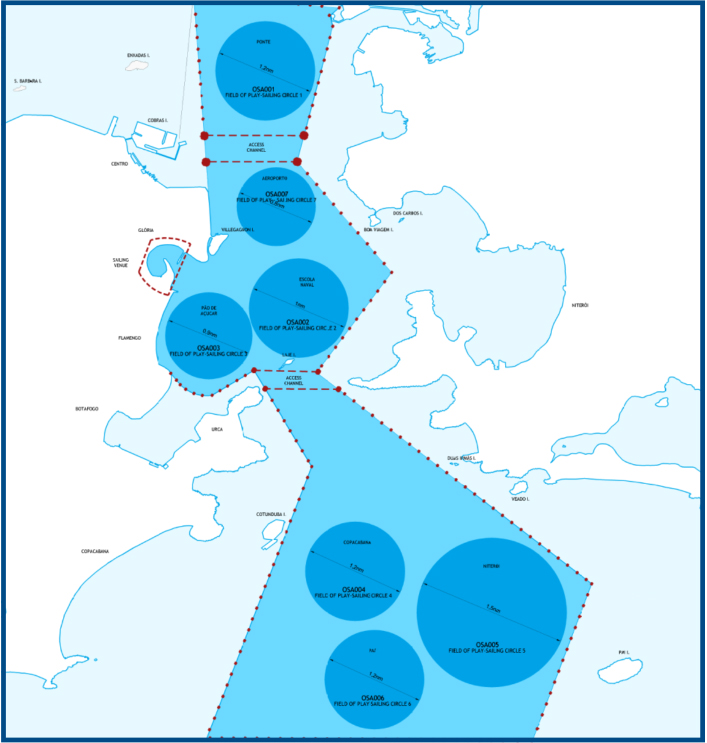
\includegraphics[width=0.6\textwidth]{16_OG_RaceAreasNOR.jpg}
  \caption{Sailing Races Areas. Olympic Games Rio 2016 \cite{instr_rio}.}
\label{fig:olymp_areas_rio} 
\end{figure}

\begin{figure}[ht]
  \centering
  \subfloat[Trapezoid Course ] {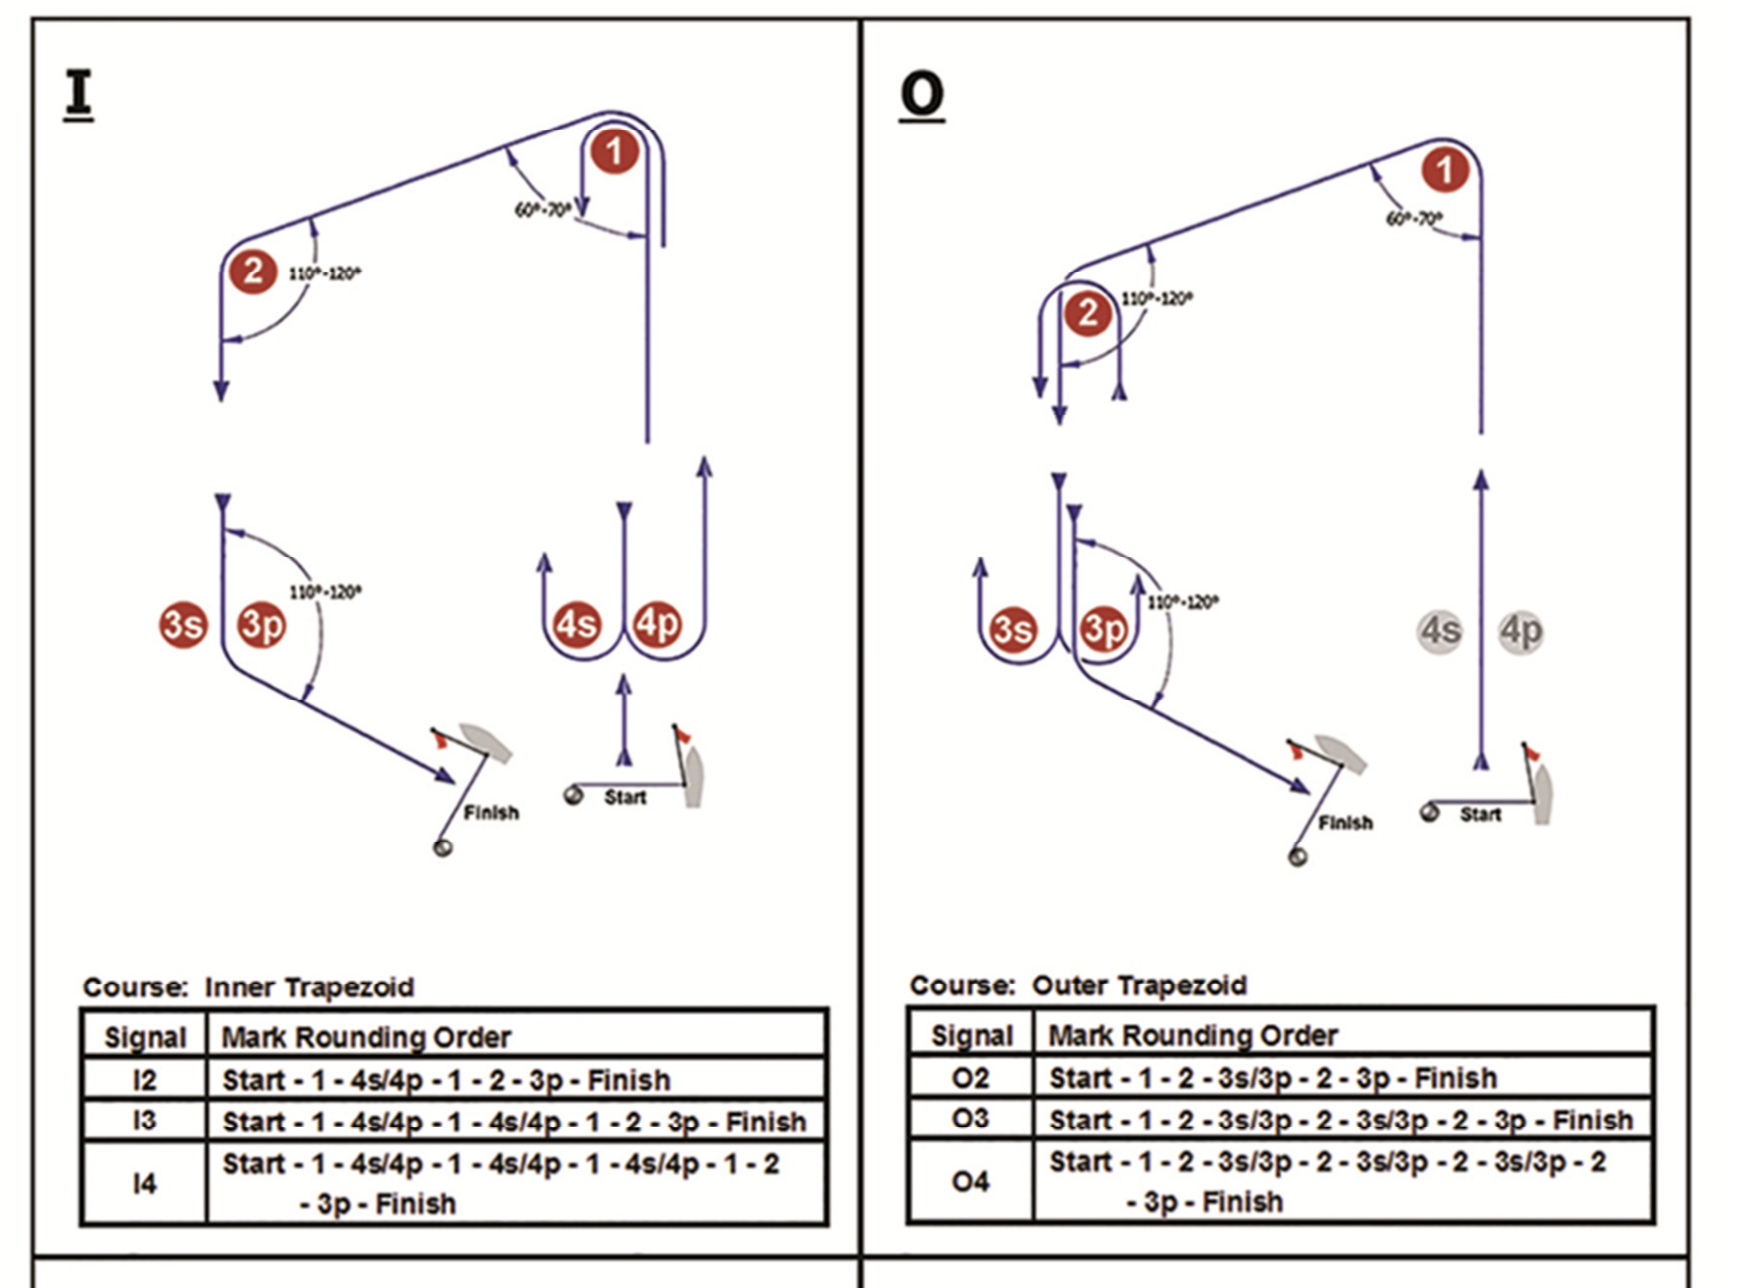
\includegraphics[width=0.53\textwidth]{trap_course.png}\label{fig:trap_c}}
  \hfill
  \subfloat[Windward / leeward course] {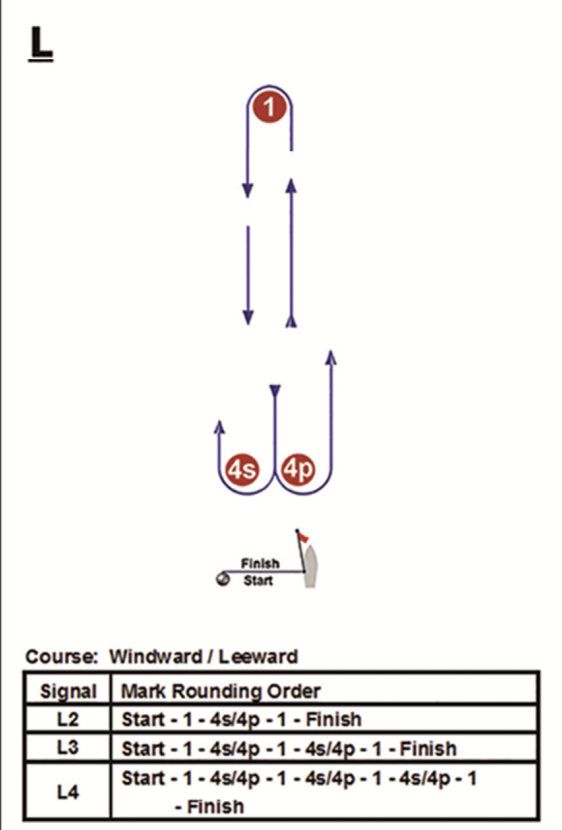
\includegraphics[width=0.25\textwidth]{l_w.png} \label{fig:wl_c}}
  \caption{Types of courses \cite{instr_rio}.}
\label{fig:typecourses} 
\end{figure}

The direction of the boat in respect to the wind determines the type of maneuvers and trajectory that must be followed. For example, the first leg of the trapezoid course runs against the wind and boats cannot displace towards it. The maneuvers used in this condition is shown in figure \ref{fig:tacking}, the trajectory forms a zig-zag pattern that can be started on the left- or on the right-hand side and each change on the heading direction is known as a tack. \par 

Even when the trajectory looks symmetrical, it is important to remember that the wind is not constant all the time and because during the competition, it is only allowed to have a maximum shift of 10 \degree \cite{race_pol}. It is important to understand how this shift affected the course, therefore the time of the course. So far there is no evidence to accept or reject this symmetric condition. This raises the question of \textit{which direction should be taken when the boat has to run against the wind}, in other words, \textit{which is the path with the minimal time to follow?}. \par \noindent
To answer this question athletes and coaches rely on their previous knowledge and experience to decide which is the starting direction. This previous knowledge is based on geographical characteristics around the area of the course and exposure to the site. Top athletes for the Olympic Games train in the site at least one year before the event.\par 
\begin{figure}[ht]
  \centering
  \subfloat[Tacking Maneuver \cite{denny2009float}.] {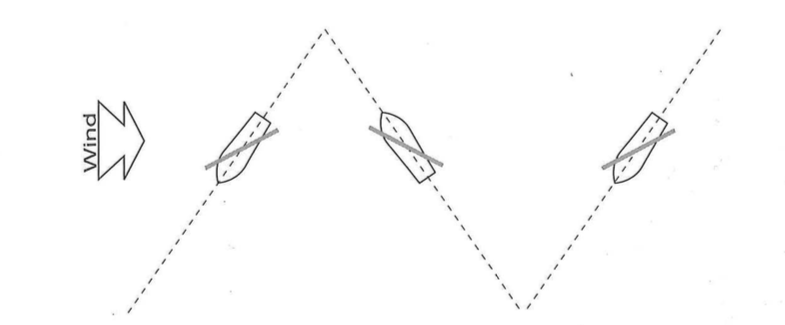
\includegraphics[width=0.65\linewidth]{tacking.png}\label{fig:tacking}}
  \hfill
   \centering
  \subfloat[Tacking maneuver]{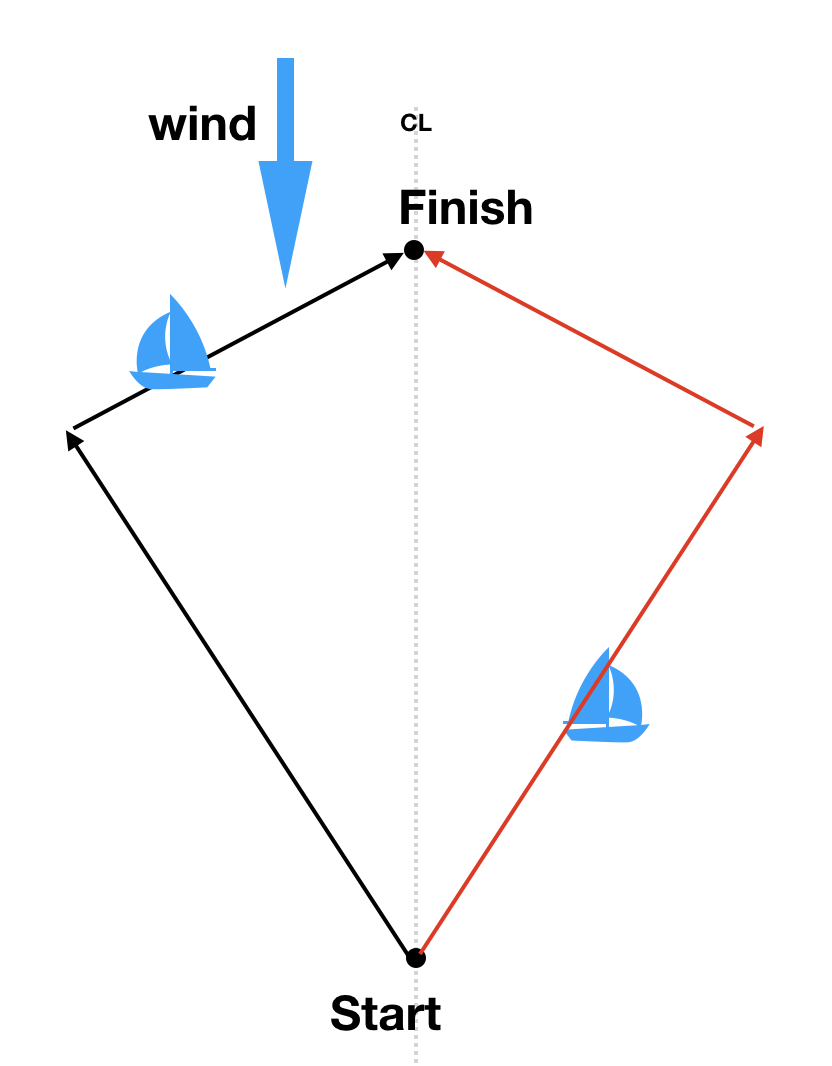
\includegraphics[width=0.3\linewidth]{images/upwind_sym.png}\label{tack_jib}}
  \caption{Tacking maneuver against the wind.}
\label{fig:tack_against_wind} 
\end{figure}

\section{Weather Forecast}
A weather forecast is calculated by supercomputers and updated every certain time according to the regions, usually every three hours. Due to its complexity different agencies and governments have developed models to predict the weather in global terms, so that local predictions could be made. This local predictions take into account the global model and adjusted according to local measurements allowing them to be updated every hour with a grid resolution of 3km by 3km \cite{warner2010numerical}. \par

Uncertain weather is a typical condition that yacht competitions and maritime transportation have to manage. In the case of yacht competitions, courses could take days, weeks or even months; like the \textit{Volvo Ocean Race}, which is an around the world. The path planning for this kind of boats has been researched especially by maritime and logistics sciences, a less number of publications can be found for yacht races and autonomous vehicles, and just a few numbers of researches refer to Olympic races. \par  

 Olympic races have a duration of maximum one hour inside a grid of size 2km by 2km and local forecast is updated every hour within a grid of 3km by 3km. Because of this, the information that coaches and athletes can access previously to the race does not match the characteristics and needs for them at first instance.\par
 Short course and long courses races are different. Short courses, for example, are more sensitive to random fluctuations \cite{philpott2001optimising}. Furthermore, the direction to take at the beginning of the competition could be the optimal just for a couple of minutes but not for the whole race. Time on Olympic sailing classes is critical to winning, but at the same time, a higher resolution on time and space for the weather is more costly in terms of computation effort for weather and the minimal time trajectory processing. The \textit{impact of a fine resolution vs a coarse on the time trajectories is unknown}. In the other hand, it is also unknown \textit{how small this resolution should be} in order to be significant for the  race.\par
 
 \section{The Aim of the Research}
This research proposes an algorithm to model sailing trajectories shaped by wind for Olympic Classes which %more specific for Laser (dinghies) competitions %and optimize it to obtain the minimal time for the Laser (Olympic class). 
can answer the question, \textit{Which is the optimal sailing route shaped by wind for the Laser (Olympic class) when the time and spatial resolution is set constant: every hour and every 10 minutes. Which resolution is the most representative?}. The study suggests that the sensibility of the optimal route due to changes in the wind field and starting direction can define zones and shape the trajectory for minimal time paths. \par 

Moreover, it demonstrates the effects of 3 different time steps and spatial resolutions on the resulting trajectories with its times. This will be done by means of experiments using the optimization of the algorithm proposed. The results(simulations) obtained can be compared against the measurement data of the selected race. In this way, it is possible to identify the size of the differences and quantify the effect of the uncertain weather over the trajectory and times.\par 
%In other words,%the critical variables influenced by the wind that determine it.
%the study seek 
%To answer the question, What is the optimal sailing route for the Laser (Olympic class) shaped by wind. The objective is to analyze the sensibility of the optimal route due to changes on the wind field and start times. This will determine the zones and the shape trajectory of the optimal path. 
%and conditions that shape not only the optimal but the least route also. 
%To answer this question first, the physical model of yachts was reviewed. Despite the similarities between dinghies(Laser boats) and yachts, the physical model was adapted by adding two coefficients related with sails which indicate%the research focusing on dinghies is significantly lower as consequence adaptations have been made to represent
%how different is steering a dinghy from a yacht. Moreover, these adaptations are reflected on the %These adaptations are related with the
%Velocity Prediction Polar (VPP)diagram. By using the VPP and the wind intensity is possible to set the direction at which the dinghy reach is maximum velocity respect to the wind. This approach is known as Velocity Made Good (VMG).%  and to more specific and the use of sails
%Despite the similarities between dinghies and yachts, the research focusing on dinghies is significantly lower as consequence adaptations have been made to represent how it is steering, one of this is related with the VPP's and the use of sails. The same situation happens when the topic of research is related with optimal routes.  Since Olympic sailing is focused on the seamanship, the understanding of physical principals intends to provide or reveal hints that helps them to train and contest effectively regardless the location and routes. \newline

 \section{Terms, conditions, and limitations}
 %This report asses them 
%%these portable designs %the three concepts  

The algorithm developed is limited to dinghies, the smallest and one of the most used boats on the Olympic classes. More specific, the Laser Class with motion over the XY plane. The 2D model proposed was validated by comparing the results of the simulations obtained against the results Laser races located at Hyères, France during 2018.\par \noindent The experiments to see the effects of the time step on the time and trajectory are the three wind conditions: first, a constant wind intensity and direction along the area of the route; the second, considers a forecast wind field as time-space-dependent variable changing every 10 minutes over 1 km by 1km grid size without current and neglecting the wave disturbances and twisting effects on the sail; the last test %condition 
uses the wind measurements taken at 20 Hz during the competition. The algorithm developed is implemented on MATLAB\textsuperscript{\textregistered} and the optimization tool used is \cite{MatlabOTB}.\par 

Olympic Classes like the dinghy is not a widespread research topic. Besides most of the findings related to path optimization for boats are related to cargo ships and vessels, where the main objective is to minimize fuel costs because this ship can be set to navigate at a constant speed. A smaller amount of researches but more related to sports are the ones related to yachts; the influence of the wind is not the same as for the Olympic Classes. \par \noindent 
Another consideration is the movement of the sailor which was not considered as a variable since it was assumed that the athlete is skilled enough to keep the equilibrium of the boat and maximize speed without further complications. In the case of the crew weight, the simulations used the weight proposed by \cite{laser_opt}, which is between	55 and 70 kg.\par 

 \section{Report Structure}
The report is set as follows: chapter 2 refers to basic concepts and physics of sailboat; the forces and equation that governs its motion in general. The validation of the model, and how the wind model is integrated is reviewed in chapter 3. In chapter 4, the optimizer algorithm is explained as well as how the model is implemented with required modifications for the purposes of this research. The obtained results are analyzed in chapter 5; and finally, the conclusions and recommendations are described in chapter 6.\par 

%has been considering in the development of methods for the optimal path.
%The random fluctuation over the time is more sensitive on short courses rather long coursed.
%Taking good decisions on time depends on: the available data and processing time. The processing time refers to the time it takes to converted the available data into meaningful information. These two variables have been approaching by Different researchers to obtain 




%Because of this Philpott \cite{philpott2001optimising} describe a method for each condition to figure out the optimal path.  The weather variables in a short courses were considered to have a minimum spatial variation, although they enclose a random component due to its dependence over time.\\


%With this method the area and time have to being discretize, more over the it consider different states or possibles angles at which the wind will be directed. Which means that each location has to evaluate each of the states and find the optimal path among  \textit{n} stages.  The larger or the smaller the the discretization the more locations to solve according each stage, which seem that the computational effort will grow considerably since each leg has to be evaluated.  The paper does not mention the computational effort nor the difference of time that can be achieve by using it.Philpott \cite{philpott2001optimising}


